%% entwurf.tex
%% $Id: entwurf.tex 61 2012-05-03 13:58:03Z bless $
%%

\chapter{Entwurf}
\label{ch:Entwurf}
%% ==============================
%In diesem Kapitel erfolgt die ausführliche Beschreibung des eigenen
%Lösungsansatzes. Dabei sollten Lösungsalternativen diskutiert und
%Entwurfsentscheidungen dargelegt werden.
In diesem Kapitel werden die Features erklärt, die grundlegend notwendig sind, sowie die, die sich während der Entwicklung ergeben haben und vom Kunden gewünscht wurden.

%% ==============================
\section{Ideen}
%% ==============================
\label{ch:Entwurf:sec:1.Konzept}
\paragraph{Grundlegende Features}
 Diese grundsätzlichen Features entsprechen dem ursprünglichen Prototypen, der in der Abbildung \ref{fig:Prototyp} zu sehen ist, des Spiels, dadurch konnten die implementierten Regeln getestet und durch weitere Ideen erweitert werden.
 	\begin{itemize}
 		\item Spielbrett, mit einer Größe von 8x8 und fix in der Szene verankert
 		\item Schwarze und weiße/graue Kreise als Spielsteine
 		\item Zwei Spieler können per Klick auf einen Stein und auf ein Feld Spielsteine bewegen
 		\item Hervorheben der möglichen Positionen
 	\end{itemize}
\begin{figure}[h]
	\centering
	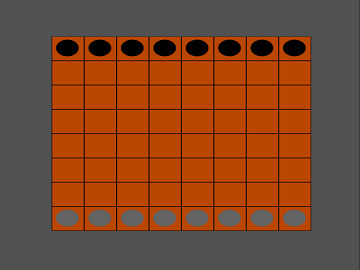
\includegraphics{img/Prototyp}
	\caption{Prototyp}
	\label{fig:Prototyp}
\end{figure}
 \paragraph{Erweiterte Features nach Testen der Logik}
 Die erweiterten Features wurden nach ausgiebigem Testen der grundsätzlichen Features und der implementierten Logik hinzugefügt.
 \begin{itemize}
 \item Künstliche Intelligenz als Gegenspieler
 \item Pausenmenü mit Neustart-, Beenden- und Start-Button
 \item Dynamisch generiertes Spielfeld für unterschiedliche Größen des Spielbretts
 \item Slider um die Punkteverteilung der künstlichen Intelligenz zu regulieren
 \item Touch-Unterstützung, da beim Landesmuseum ein Touchscreen verwendet wird, soll das Spiel die Bedienung ohne Maus und Tastatur unterstützen
 \item Simple Kreise durch Sprites von historisch verwendeten Spielsteinen ersetzen
\end{itemize}


\paragraph{Zusätzliche Features bei Übergabe an Kunden}
Nachdem das zuvor konzeptionierte Spiel dem Landesmuseum Birkenfeld zugeschickt wurde, haben sich die folgenden noch zusätzlich benötigten Features herausgestellt:
\begin{itemize}
	\item Unterschiedliche Schwierigkeitsgrade anstatt Slider im Spiel gegen die KI, da diese nicht so intuitiv verstanden wurden
	\item Zweite KI soll zuschaltbar sein um Spiel zu simulieren
	\item Neustart- und Beenden-Buttons auf den Spielbildschirm verschieben	
\end{itemize}


\paragraph{Benötigte Grafiken}
Zur Umsetzung von Latrunculi wurden folgende Sprites genutzt:
\begin{itemize}
	\item Spieler 1 als Muscheln
	\item Spieler 2 als Steine
	\item Quadratische Zellen als einzelne Felder des Spielbretts
	\item Quadratische Zellen mit Hervorgehobenen Rändern als Rückmeldung welche Bewegung möglich ist
\end{itemize}

\paragraph{Nötige Technologien}
\begin{itemize}
	\item Unity 2019.3.14f als Engine
	\item C\# für die verwendeten Skripte
	\item Visual Studio 2019 als Entwicklungsumgebung 
	\item GIMP zum erstellen und bearbeiten von Sprites
\end{itemize}

\paragraph{Künstliche Intelligenz}
Um das Spielen auch alleine zu ermöglichen wurde auf Basis des MiniMax-Algorithmus eine künstliche Intelligenz entwickelt gegen die ein Spieler antreten kann. Hierbei können unterschiedliche Schwierigkeitsgrade ausgewählt werden, indem die Punkteverteilung des Algorithmus und die Tiefe, die dieser berechnen soll, angepasst werden. Außerdem wurde für Vorführungen im Museum eine zweite KI mit einer eigenen Punkteverteilung hinzugefügt um das Spiel auch als Simulation laufen lassen zu können.

%% ==============================
%%\section{Abschnitt 2}
%% ==============================
%%\label{ch:Entwurf:sec:Abschnitt2}

%% ==============================
%%\section{Zusammenfassung}
%% ==============================
%%\label{ch:Entwurf:sec:zusammenfassung}

%%Am Ende sollten ggf. die wichtigsten Ergebnisse nochmal in \emph{einem}
%%kurzen Absatz zusammengefasst werden.

%%% Local Variables: 
%%% mode: latex
%%% TeX-master: "thesis"
%%% End: 
